% ============================================================
% chapters/nonvf.tex
% Merge of:
%   (S) nonvf-paper-succint/main.tex -- "Scoring agents for what
%       is neither verifiable nor falsifiable" (AAMAS format);
%       provides the narrative backbone (Sections 1-3, 5, 6).
%   (L) nonvf-paper/main.tex -- "Betting on what is neither
%       verifiable nor falsifiable" (arXiv:2402.14021); its
%       Framework + Results sections become Section 4, its
%       appendix becomes subappendix A (using the fuller text of
%       nonvf-paper-succint/stuff.tex, which is a superset of it).
% Chapter-local macros: macros/nonvf.tex (agent notation, \Prob
% override, etc. -- see the header of that file for the merge
% decisions).
% ============================================================

\chapter{Scoring agents for what is neither verifiable nor falsifiable}
\label{ch:nonvf}

\chaptersource{This chapter is based on the paper \emph{``Scoring agents for what is neither verifiable nor falsifiable''} (Abhimanyu Pallavi Sudhir and Long Tran-Thanh, University of Warwick; AAMAS format) and on its longer companion version \emph{``Betting on what is neither verifiable nor falsifiable''} (arXiv:2402.14021). The succinct version supplies the chapter's narrative; the long version's concrete program-market construction, its results and its appendix on Garrabrant induction are folded in as Section~\ref{nonvf:sec:market} and Appendix~\ref{nonvf:app:garrabrant}.}

\chapterabstract{Classical methods to elicit probabilities of events, such as proper scoring rules and prediction markets, are only useful when the events are either \emph{verifiable} (if true, will eventually be revealed as true) or \emph{falsifiable} (if false, will eventually be revealed as false). However, both probability theory and first-order logic allow for events/sentences that do not fit these criteria -- a simple example of such a sentence is ``all men are mortal''. In this paper, we propose a mechanism to elicit probabilities on such sentences, by treating them as bets on the outcome of a ``verification-falsification game''. Our work thus acts as an alternative to the existing Garrabrant induction framework for logical uncertainty, and is related to concepts such as game semantics and Debate.}

\section{Introduction}
\label{nonvf:sec:intro}

\emph{Incentivizing (human or AI) agents to truthfully report their beliefs} is a problem of central importance in both machine learning and economics \cite{savageElicitationPersonalProbabilities1971,gneitingStrictlyProperScoring2007}. One standard approach to this is \emph{proper scoring rules}: e.g. in logarithmic scoring \cite{goodRationalDecisions1952}, an agent is given reward $\log(p)$ for reporting probability $p$ to a binary event which turns out to be true. Another approach is a \emph{prediction market} \cite{hansonLogarithmicMarketScoring2002, hansonCombinatorialInformationMarket2003, beygelzimerLearningPerformancePrediction2012, conitzerPredictionMarketsMechanism2012}: here, an asset contingent on the event is offered to the agent, and the agent's ``fair price'' (the price at which it neither buys nor sells), is its subjective probability -- for example, if you believe there is a 70\% chance of Jeb Bush winning the 2028 election, you will pay \$0.70 for the asset ``pays \$1 if Jeb wins; \$0 otherwise''.

All of these mechanisms depend on the ground truth of the sentence being eventually revealed. At most, we can generalize them to \emph{verifiable sentences} (sentences whose ground truth will be revealed if they are true, e.g. ``Bob will eventually die'', verified by Bob dying) or \emph{falsifiable sentences} (sentences whose ground truth will be revealed if they are false, e.g. ``Bob will never die'', falsified by Bob dying) -- for the latter, we may pay the agent \$1 upfront, to be returned upon the sentence being falsified.\footnote{Such an asset may be traded on a market as defined by standard mechanisms such as continuous double auctions or logarithmic market scoring. For the details of such algorithms see \cite{conitzerPredictionMarketsMechanism2012, hansonLogarithmicMarketScoring2002, hansonCombinatorialInformationMarket2003} or real-life prediction markets such as PredictIt, SMarkets, or the play-money market Manifold.} % (L) footnote from the long version's introduction

Although falsifiability occupies a central role in the imagination of philosophers \cite{thorntonKarlPopper2023}, a much wider class of sentences are treated in science and in common practice, and are allowed by first-order logic (FOL) and probability theory. In FOL, we may let $\Delta_0=\Sigma_0=\Pi_0$ denote sentences that will resolve in known time, $\Sigma_{n+1}$ denote sentences of the form $\exists x\ P(x)$ where $P(x)$ is $\Pi_n$, and $\Pi_{n+1}$ denote sentences of the form $\forall x\ P(x)$ where $P(x)$ is $\Sigma_n$. Thus verifiable sentences are $\Sigma_1$, and falsifiable sentences are $\Pi_1$, but all sentences further up the arithmetical hierarchy, $\Sigma_{n>1},\Pi_{n>1}$ are \emph{neither verifiable nor falsifiable} (non-VF)\noop{Similarly in probability theory, if we let $\{X_1,X_2,\dots\}$ be a set of base events which will be observed within finite time, then countable unions of subsequences $\bigcup_{i} X_{i_j}$ denote verifiable sentences (observing any true $X_i$ verifies it) while countable intersections $\bigcap_{i} X_{i_j}$ denote falsifiable sentences (observing any false $X_i$ falsifies it). But sentences higher up, e.g. $\bigcup_i\bigcap_j X_{f(i, j)}$ are non-VF.}. Examples of non-VF sentences:
\begin{itemize}
  \item ($\Pi_2$) ``all men are mortal'' ($\forall\,\mathrm{man}\,\exists t,\operatorname{dies}(\texttt{man}, t)$)
  \item ($\Sigma_2$) ``The US will eventually permanently annex Greenland'' ($\exists t,\forall s>t,\,\texttt{greenland\_in\_us\_at\_time}(s)$)
  \item ($\Pi_3$) ``Long-run GDP growth will be expontential with rate 2\%'' ($\forall\varepsilon>0,\exists t, \forall s>t, \,|\left(\texttt{GDP}(t)/\texttt{GDP(0)}\right)^{1/t}-1.02|<\varepsilon$)
\end{itemize}

In all of these cases, there is no source of ground truth that lets us resolve the question with certainty: verifying ``all men are mortal'' would need checking an infinite number of men who will ever be born; falsifying it would require finding an immortal man, but proving him to be immortal will take infinite time. Yet these are all very common sentences, which we may find it useful to have a probability estimate on.

% (L) the following sentence and Fig are from the long version's introduction.
In this paper we will be concerned with designing prediction markets for sentences in \emph{first-order logic} (FOL), though our results may also be straightforwardly generalized to a hyperarithmetical logic up to any computable ordinal (see e.g. \cite{pohlersComputabilityTheoryHyperarithmetical1999, ashComputableStructuresHyperarithmetical2000, moschovakisDescriptiveSetTheory2009, kechrisClassicalDescriptiveSet1995} for standard introductions); Fig~\ref{nonvf:fig:fol} shows the ``arithmetical hierarchy'' of First-Order Logic sentences.

\begin{figure}
    \centering
    \usetikzlibrary{arrows}
\usetikzlibrary{positioning}
\pgfmathsetmacro{\myw}{3.6}
\pgfmathsetmacro{\myh}{2.6}
\pgfmathsetmacro{\mys}{0.25}
\newlength{\mypad}
\setlength{\mypad}{8pt}
\newlength{\mylsl}
\setlength{\mylsl}{-1pt}
\newlength{\mylsg}
\setlength{\mylsg}{1pt}

\begin{tikzpicture}[line width =1pt, scale=0.9]

\draw (0,0) -- (0,3*\myh+4*\mys);
\draw (\myw,0) -- (\myw,3*\myh+4*\mys);
\node[] at (\myw/2,3*\myh+4*\mys){$\dots$};
\draw node[above = \mypad, anchor = north east]{$\Delta_0$} (0,0) -- (\myw,0) node[above = \mypad, anchor = north west]{$\Delta_0$};
\draw (0,0) -- (\myw,\myh) node[above = \mypad, anchor = north west]{
    \begin{tabular}{l}
        $\Pi_1$ \vspace{\mylsg}\\
        ``Bob will die'' \vspace{\mylsg}\\
        ``all swans are white'' \vspace{\mylsg}\\
        ``$P$ does not halt''
    \end{tabular}};
\draw (\myw,0) -- (0,\myh) node[above = \mypad, anchor = north east]{
    \begin{tabular}{r}
        $\Sigma_1$ \vspace{\mylsg}\\
        ``Bob will die'' \vspace{\mylsg}\\
        ``there is a white swan'' \vspace{\mylsg}\\
        ``$P$ halts''
    \end{tabular}};
\draw (0,\myh+\mys) -- (\myw,2*\myh+\mys) node[above = \mypad, anchor = north west]{
    \begin{tabular}{l}
        $\Pi_2$ \\
        ``all men are mortal'' \vspace{\mylsg}\\
        ``all swans will lay\vspace{\mylsl}\\
        a white egg'' \vspace{\mylsg}\\
        ``there are an infinite\vspace{\mylsl}\\
        number of primes''
    \end{tabular}};
\draw (\myw,\myh+\mys) -- (0,2*\myh+\mys) node[above = \mypad, anchor = north east]{
    \begin{tabular}{r}
        $\Sigma_2$ \\
        ``there is an immortal man'' \vspace{\mylsg}\\
        ``there is a swan that\vspace{\mylsl}\\
        always lays brown eggs'' \vspace{\mylsg}\\
        ``there are finitely\vspace{\mylsl}\\
        many perfect numbers''
    \end{tabular}};
\draw (0,2*\myh+2*\mys) -- (\myw,3*\myh+2*\mys) node[above = \mypad, anchor = north west]{
    \begin{tabular}{l}
        $\Pi_3$ \vspace{\mylsg}\\
        ``$x_n$ converges to 2''
    \end{tabular}};
\draw (\myw,2*\myh+2*\mys) -- (0,3*\myh+2*\mys) node[above = \mypad, anchor = north east]{
    \begin{tabular}{r}
        $\Sigma_3$ \vspace{\mylsg}\\
        ``$x_n$ does not converge to 2''
    \end{tabular}};
\end{tikzpicture}
    \caption{The ``arithmetical hierarchy'' of FOL sentences. A $\Sigma_{n+1}$ sentence is of the form $\exists x,p(x)$ where $p$ is $\Pi_n$; a $\Pi_{n+1}$ sentence is of the form $\forall x,p(x)$ where $p$ is $\Sigma_n$. In logic, the lowest level of the arithmetical hierarchy $\Delta_0=\Sigma_0=\Pi_0$ are sentences of the form $f(n)=0$ where $f$ is a primitive recursive function, but this formalism may be extended to empirical truths that will be revealed at a fixed time.}
    \label{nonvf:fig:fol}
\end{figure}

There are two common ways that market-creators attempt to work around this limitation in practice\footnote{this can be attested by a brief skim through the front pages of popular forecasting platforms such as Polymarket and Manifold Markets}:
\begin{itemize}
\item asking about \emph{finite-horizon} versions of non-VF sentences (e.g. ``Greenland will be annexed and remain part of the US until at least 2100''), or
\item asking whether the sentence will be \emph{proven} (either via formal proofs or appealing to the authority of ``credible sources'').
\end{itemize}
The pitfalls of the first method are explained in Section~\ref{nonvf:sec:impossible}; the most refined example of the second method is \emph{Garrabrant induction} \cite{garrabrantLogicalInduction2020}, described in Section~\ref{nonvf:sec:related}.

We propose a new framework for eliciting probabilities on non-VF sentences: we allow agents to bid for the opportunity of playing the \emph{verification-falsification game} for that sentence, and take the value of the bid to be their implied probability for that sentence. {There are limitations to our mechanism, such as when one side of the game is much easier to play than the other, and we outline some ideas on how these may be overcome.}


\subsection{Related work}
\label{nonvf:sec:related}

\textbf{Logical uncertainty.} Our work may equivalently be understood as a formalism for \emph{logical uncertainty} (see \cite{halpernReasoningUncertaintySecond2017} for a summary of work in the area), i.e. the problem of assigning probabilities to mathematical sentences in some language $\mathcal{L}$ (which could be a language of FOL sentences). The most relevant work in this domain is \emph{Garrabrant induction} \cite{garrabrantLogicalInduction2020}, which constructs a prediction market for each mathematical sentence that pays off when it is proven by a theorem-enumerator for some theory $\mathcal{T}$ over $\mathcal{L}$.\footnote{to avoid simply being a prediction market for the provability of a sentence, they use a special accounting measure for agent wealths based on ``propositionally consistent worlds'' -- e.g. fixing the combined price of $P$ and $\lnot P$ at \$1 -- which allows them to extend this framework to sentences independent of $\mathcal{T}$.} \draft{A detailed description of the Garrabrant induction construction, and of its limitations for our purposes, is given in Appendix~\ref{nonvf:app:garrabrant}.}

There are two limitations of this framework for our purposes. First: while mathematical theories can easily prove non-VF sentences (e.g. $\forall x,\exists y>x,\,\texttt{prime}(y)$) there is no analogous theory in the real world that we are aware of (``observation'' only proves VF sentences, as discussed). Second: it is philosophically unsatisfying to have probabilities for logical sentences be completely dependent on a mathematical theory, and change when the theory is strengthened or weakened (e.g. by the addition of a G\"odel sentence).

Logical uncertainty has also been discussed in the Bounded Rationality literature e.g. in \cite{halpernAlgorithmicRationalityGame2014,halpernDontWantThink2011,oesterheldTheoryBoundedInductive2023}; however this has typically focused on toy examples based on VF sentences, e.g. betting on the trillionth digit of $\pi$, etc., % (L) closing clause from the long version's corresponding paragraph:
as the games therein have to pay out a reward at a fixed point depending on the answer to the question.

\textbf{Game semantics.} The \emph{verification-falsification game} we use is from Hintikka's \emph{game semantics} \cite{hintikkaGameTheoreticSemantics1997}, which we will discuss in Section~\ref{nonvf:sec:framework}. Game semantics has since been expanded into the field of \emph{computability logic} \cite{japaridzeBeginningWasGame2009,japaridzeSurveyComputabilityLogic2015}, which may be the most natural setting to formulate some of our more speculative ideas about probability theory, described in Sec~\ref{nonvf:sec:conclusion}.

\textbf{Debate.} AI Debate \cite{irvingAISafetyDebate2018} considers sentences $P$ that can be expressed like $\exists x_1\ \forall x_2\ \dots \exists x_n,H(x_1,\dots x_n)$ (more generally any $\Sigma_n$ or $\Pi_n$ form in $H$) where $H$ is some ``human-computable function'', and argues that AIs can be trained to answer such questions correctly via \emph{debate} judged by a human\footnote{in particular, supervised learning can train an AI to learn to answer $\Delta_0$ questions, and reinforcement learning can train an AI to learn to answer $\Sigma_1$ questions}. This is quite similar to our setting, and debate is analogous to the verification-falsification game, except that physical ground truth is replaced by human-computability (or polynomial-computability as they hypothesize). We hope our work can serve as a valuable intuition pump for debate.

\textbf{AI Forecasting.} There has recently been a surge of interest in AI forecasters \cite{zouForecastingFutureWorld2022, schoeneggerLargeLanguageModel2023,yanAutoCastEnhancingWorld2023, halawiApproachingHumanLevelForecasting2024a, schoeneggerWisdomSiliconCrowd2024} -- in particular, recent works such as \cite{sudhirConsistencyChecksLanguage2024} have investigated the \emph{propositional consistency} of AI forecasters, i.e. whether the probabilities they give satisfy basic rules of probability theory like $\Prob{P}+\Prob{\lnot P}=1$. Similarly our work can be understood as asking how we can incentivize or evaluate forecasters respecting the ``continuity of probability'' rules $\Prob{\bigcup P_i}=\lim_{n\to\infty}\bigcup_{i<n}\Prob{P_i}$ and $\Prob{\bigcap P_i}=\lim_{n\to\infty}\bigcap_{i<n}\Prob{P_i}$.

\section{Impossibility theorem}
\label{nonvf:sec:impossible}

One apparent solution may be to approximate FOL sentences with long finite horizons -- i.e. approximate $\exists x,\forall y, P(x,y)$ with a bounded quantification $\exists x<G,\forall y<G, P(x,y)$ for some large $G$, which is a $\Delta_0$ sentence as it can be determined by enumerating $G^2$ tuples. One might also consider a sequence of such bounded quantification ``approaching'' the FOL sentence, e.g. consider the asset that on day $t$ is equal to (can be exchanged for) $\exists x< t,\forall y< t, P(x,y)$. A simple counter-example to this approach is: $\exists x,\forall y,x\ge y$, illustrated in Fig~\ref{nonvf:fig:checkerboard}: for any finite $G$, the corresponding bounded quantification is true (take $x=G$), but the sentence is false.

% (L) two-panel figure from the long version (superset of the succinct
% version's single-panel figure; caption from the long version).
\begin{figure}
    \centering
    \begin{subfigure}{0.45\textwidth}
        \centering
        \usetikzlibrary{arrows}
\usetikzlibrary{positioning}

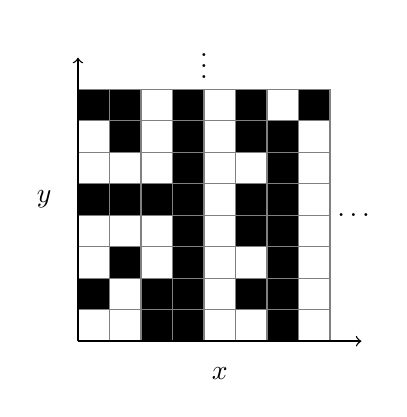
\begin{tikzpicture}[line width =0.5pt, scale=0.4]

\draw[gray] (0,0) grid (8,8);
\foreach \x/\y in {0/1, 0/4, 0/7, 1/2, 1/4, 1/6, 1/7, 2/0, 2/1, 2/4, 3/0, 3/1, 3/2, 3/3, 3/4, 3/5, 3/6, 3/7, 5/1, 5/3, 5/4, 5/6, 5/7, 6/0, 6/1, 6/2, 6/3, 6/4, 6/5, 6/6, 7/7}
    \filldraw[fill=black, draw=gray] (\x,\y) rectangle ++(1,1);
\draw[->] (0,0) -- (9,0) node[midway, below=6pt]{$x$};
\draw[->] (0,0) -- (0,9) node[midway, left=6pt]{$y$};
\node[] at (4,9){$\vdots$};
\node[] at (8.75,4){$\dots$};
\end{tikzpicture}
        \label{nonvf:fig:checkerboard1}
    \end{subfigure}\hfill%
    \begin{subfigure}{0.45\textwidth}
        \centering
        \input{figs/nonvf/checkerboard2}
        \label{nonvf:fig:checkerboard2}
    \end{subfigure}
    \caption{Shading $P(x,y)$ as a checkerboard, the $\Sigma_2$ sentence $\exists x,\forall y, P(x,y)$ can be interpreted as ``there is an infinite black column''. Left: an arbitrary example; Right: the example of $P(x,y):=x\ge y$, where the $\Sigma_2$ sentence is false, yet it is true for every ``finite window''.}
    \label{nonvf:fig:checkerboard}
\end{figure}

Theorem~\ref{nonvf:thm:nogo} shows there is no general mechanism to give a proper scoring rule or an equivalent asset for any non-VF sentence:

\begin{definition}[Asset and scoring mechanisms]
  An asset mechanism is a computable real-valued function $v:\Nats\times\Props\to\Reals$ such that $\lim_{t\to\infty}v(t,P)=1$ if $P$ and $0$ if $\lnot P$. Let $s:[0,1]\to\Reals$ be a proper scoring rule e.g. $s(p)=\log(p)$. A scoring mechanism for proper scoring rule $s$ is a computable real-valued function $\sigma:\Nats\times\Props\times[0,1]\to\Reals$ such that $\lim_{t\to\infty}\sigma(t,P,p)=\{s(p)\text{ if }P\text{ else }s(1-p)\}$.
  \label{nonvf:def:mechanisms}
\end{definition}

\begin{theorem}[Impossibility theorem]
  If $\Props$ is the set of FOL sentences, then there does not exist either an asset mechanism nor a scoring mechanism.
  \label{nonvf:thm:nogo}
\end{theorem}
\begin{proof}
  The statements $\lim_{t\to\infty}v(t,P)=1$ and $\lim_{t\to\infty}\sigma(t,P,p)=s(p)$ are both $\Pi_3$ for any $P, p$; thus for them to be equivalent to $P$ for all $P$ would violate Tarski's theorem.
\end{proof}

\draft{The long version of the paper states this result with a sharper hypothesis: neither mechanism exists as soon as $\Props$, the class of propositions considered, includes at least $\Sigma_4$ or $\Pi_4$ sentences.}

\section{Ranged VF games}
\label{nonvf:sec:framework}

In this paper, we propose a game-theoretic solution motivated by the following intuition. If you believe that ``all men are mortal'', then you should agree to the following bet: I can choose the name of any man, and you must be able to give the year by which he will be dead. If you succeed, you win the bet; if you don't, I win. This is formally analogous to the classic Verification-Falsification (VF) game from \cite{hintikkaGameTheoreticSemantics1997}, described in Def~\ref{nonvf:def:vfgame}.

\begin{definition}[Verification-Falsification game]
  To each FOL sentence $P$ we associate a sequential game between two players, the ``Verifier'' ($V$) and the ``Falsifier'' ($F$). If $P$ is $\Delta_0$, then $V$ or $F$ win \$1 if $P$ is true or false respectively. Else if $P$ is $\Sigma_n$, then $V$ goes first and if $P$ is $\Pi_n$, then $F$ goes first. The first player chooses $x\in\Nats$ as their move, and the game proceeds as the VF game for $P[x]$ (i.e. the leading bound variable substituted with $x$). Some variations:
  \begin{itemize}
  \item (\emph{ranged}) Instead of picking $x\in\Nats$ as its move, each player picks a finite set $S\in\finset\Nats$ as its move and the game proceeds as $P[S]$ , i.e. $\exists x\in S,P[x]$ if $P$ is $\Sigma_n$ or $\forall x\in S,P[x]$ if $P$ is $\Pi_n$. This eventually terminates when all the quantifications have become bounded, i.e. the sentence is $\Delta_0$.
  \item (\emph{favorable}) One of the players is ``favored'': they are allowed to go back to any earlier stage of the game, change it moves, and continue from there, as many times as it wants. This is the ``game with backward moves'' from \cite{bonnayPreuvesJeuxSemantiques2004,boyerProofTruth2012}, and has the property that if the favored player's position is provable, they have an obvious computable winning strategy (a depth-first search with backtracking).
  \end{itemize}
  \label{nonvf:def:vfgame}
\end{definition}

The \emph{ranged} VF game is original to us, and is what we use: you might believe that all men are mortal but have a probability distribution on the year any one of them will die, rather than knowing the exact date with certainty.

Observe that player policies have type $\pi:\Props\to\finset\Nats$. We may denote the $\Delta_0$ sentence produced after playing the game through as $P[\pi_V,\pi_F]$. Although the game is traditionally defined for logical sentences, it is easy tro see how this extends to probabilistic events:

\begin{definition}[FOL algebra]
  Let $\Delta_0=\Sigma_0=\Pi_0=\{B_1,B_2,\dots\}$ consist of a set algebra of base events which will be observed within finite time; $\Sigma_{n+1}$ consist of all events of the form $\bigcup_{i}X_i$ where $X_i$ is $\Pi_n$ and $\Pi_{n+1}$ consist of all events of the form $\bigcap_{i}X_i$ where $X_i$ is $\Sigma_n$. Then we will call $\Delta_0\cup\bigcup\Sigma_n\bigcup\Pi_n$ an ``FOL algebra'' over $\Delta_0$, and it is a subset of the $\sigma$-algebra generated by $\Delta_0$.
  \label{nonvf:def:probfol}
\end{definition}

We will continue to freely write $\bigcup_{i}X_i$ and $\bigcap_{i}X_i$ in the logical notation $\exists i,X_i$ and $\forall i,X_i$. We may easily speak of probabilities $\Prob{P}$ of sentences in the FOL algebra by defining a probability distribution on the base set algebra. Then we have the following result\footnote{this can be seen as a generalization of the classic statement from game semantics that the verifier or falsifier has a winning strategy if and only if the sentence is true or false respectively}:

\begin{theorem}[Value of ranged VF game]
  Assume a FOL algebra with a probability distribution $\Problem$ defined on it, and let $P$ be a sentence in this FOL algebra. Then $\Prob{P}$ is bounded between the guaranteed value of the game for the verifier and 1 minus the guaranteed value of the game for the falsifier:

  \begin{equation*}
    \sup_{\pi_V}\inf_{\pi_F}\Prob{P[\pi_V,\pi_F]} \le
    \Prob{P} \le
    \inf_{\pi_F}\sup_{\pi_V}\Prob{P[\pi_V,\pi_F]}
  \end{equation*}
  (where the $\sup$ and $\inf$ are taken over $\Props\to\finset\Nats$) We will denote each side of the inequality as $\Prob[-]{P}$ and $\Prob[+]{P}$ respectively.
  \label{nonvf:thm:supinf}
\end{theorem}
\begin{proof}
We prove this by induction on the degree of $P$. Suppose the theorem is true for $P$ up to $\Sigma_n,\Pi_n$. Then take some event $P:=\forall x, P(x)$ where each $P(x)\in\Sigma_n$:

\begin{align*}
  \Prob{P}
  &=\Prob{\bigcap_{x\in\Nats}P(x)}\\
  &=\inf_{S\in\finset\Nats}\Prob{\bigcap_{x\in S}{P(x)}}\\
  &\ge
  \inf_{S\in\finset\Nats}
    \sup_{\pi_V}\inf_{\pi_F}\Prob{
      \left(\cap_{x\in S}{P(x)}\right)[\pi_V,\pi_F]
    }\\
  &\ge \sup_{\pi_V}\inf_{S\in\finset\Nats}\inf_{\pi_F}\Prob{
    \left(\cap_{x\in S}{P(x)}\right)[\pi_V,\pi_F]
  }\\
\end{align*}

(where we have successively applied continuity of probability, the inductive hypothesis and the max-min inequality) Now note that $\left(\cap_{x\in S}{P(x)}\right)[\pi_V,\pi_F]=P[S][\pi_V,\pi_F]$, which is equivalent to $P[\pi_V,\pi'_F]$ where $\pi'_F$ is identical to $\pi_F$ except on $P$, where $\pi'_F(P)=S$. Thus:
\begin{equation*}
  \Prob{P}\ge \sup_{\pi_V}\inf_{\pi'_F}\Prob{
    P[\pi_V,\pi'_F]
  }
\end{equation*}

Which completes the first half of the inequality. The proof for the $P\in\Sigma_{n+1}$ case is identical, and the other half of the inequality is immediate from applying the first half to $\lnot P$.

\end{proof}

Several elicitation mechanisms are now immediate:

\textbf{Bidding to play.} Agents bid to play as either the verifier or falsifier of a ranged VF game for $P$. The highest bidders for each side are chosen to play against each other, and their bids are taken as estimates of the probability of $P$ and $\lnot P$. Note that the market-maker does not have to take a loss: even though this may be a negative-sum game because of potential computational costs, the total prices will still add up to at least \$1 because otherwise one of the players could just bid to take both sides and win a guaranteed total \$1.

\textbf{Double auctions.} However, it is possible for agents to overestimate their winnings and drive the total price above \$1, and this also does not give a way for agents to bid down the price of one position. We can solve this by selling multiple games via a double-auction with an order book where buy offers for the Falsifier position at price $q$ are interpreted as sell orders for the Verifier position at price $1-q$ and matched to buy orders for the Verifier position at price $p\ge 1-q$.

\textbf{Subsidized markets.} Alternatively, we may simply run one high-stakes Verification-Falsification game, retaining bidding for selecting players, but base probabilities on a separate betting market for the outcome of the game. It is possible here that the best players are not selected (e.g. due to independently wealthy players outbidding them), but an advantage is that these markets can be subsidized with arbitrary scoring rules\footnote{See \cite{hansonLogarithmicMarketScoring2002} for an introduction to market scoring rules}; traditional methods to integrate scoring rule based market makers such as \cite{agrawalUnifiedFrameworkDynamic2011, chakrabortyPriceEvolutionContinuous2015} do not work for us, as they require the market-maker to take the opposite side of every trade, which for us will require having the market-maker actively play the game.

\textbf{Training AI forecasters.} We can get our probability estimates from an AI instead of the market, by training an ``estimating agent'' $\alpha:\Props\to\finset\Nats\times[0,1]$ which outputs both a move and an estimate of its reward. The agent may then earn a combined reward for winning the game and for placing an accurate forecast. The most natural architecture for such a forecaster would be a transformer which takes input in natural or formal language and gives a sequence of integers as its output.

% ============================================================
% (L) Section 4: the long version's "Framework" and "Results"
% sections -- the concrete Garrabrant-induction-style program-
% market construction. Section title composed for the thesis.
% ============================================================
\section{A program market for VF games}
\label{nonvf:sec:market}

\begin{draftblock}
The mechanisms of Section~\ref{nonvf:sec:framework} construct the game and its associated markets abstractly. The long version of this work makes one of them fully concrete, as a Garrabrant-induction-style \emph{program market} whose participants are enumerated programs that trade on -- and play the ranged VF game for -- FOL sentences; this construction is what allows the optimality theorems below to be stated precisely. The remainder of this section is taken from the long version.
\end{draftblock}

Naturally by Theorem~\ref{nonvf:thm:nogo} this does not have the standard property expected from a traditional prediction market (that agents are incentivized to bet the price up to their subjective probability for the sentence), however it does have a closely related property that may be interpreted in terms of \emph{constructivism} in the philosophy of mathematics, as we will see.

\begin{notation*}
    Booleans are denoted as $\Bools$ representing ``false'' and ``true'' respectively. Multivariable functions may be denoted as $f:S_1\to S_2\dots S_n\to T$ i.e. with $\to$ right-associative; we may sometimes type a function $f:S\to T$ as $f:(s:S)\mapsto T$ or even $f:s\mapsto T$ like a sort of $\lambda$-notation; wherein unless otherwise specified, time denoted by $t$ belongs to $\Nats$. $\proj[TU]:S\times T\times U\to T\times U$ denotes projection; $\finset{S}$ denotes the set of finite sets of elements in $S$; for a subset $T\subseteq S$, $\compl{T}$ denotes its complement; if a set $S$ contains an element $\zero$, then $f:T\too S$ denotes a function with finite support $\supp{f}:=\preimg{f}{\compl{\{\zero\}}}:= \{x\mid f(x)\ne\zero\}$; the addition of a canonical $\zero$ element to a set $S$ is denoted by $\maybe{S}:=S\cup\{\zero\}$. We use the notation $f:T\toc S$ to denote an arbitrary partial computable function, $f:T\topt S$ to denote a function that is polynomial-time in input $t$, $f:T\tod S$ to denote a non-increasing function, and $f:T\toe S$ to denote a piecewise-constant function over a finite number of pieces, i.e. an $S$-labeled partition of $T$ (so e.g. $f:T\tode S$ denotes a function that is both non-increasing and piecewise-constant), and $\intlen{l}$ to denote the length of a clopen interval or finite union of clopen intervals $l\subseteq\Rats$. Denote by $\strings$ the set of finite strings with the infix $\concat{l_1}{l_2}$ indicating string concatenation, $\Props$ the set of FOL sentences in prenex normal form, $\Props^+:=\Props\cap\compl{\Delta_0}$ and $\Sigma=\bigcup\Sigma_n$, $\Pi=\bigcup\Pi_n$. For $n\in\Nats$ and $P\in\Props^+$, the replacement of the leading variable in $P$ by $n$ is denoted $\play{P}{n}$ (i.e. if $P:=\exists x,p(x)$ or $P:=\forall x,p(x)$ then $\play{P}{n}:=p(n)$). Let $N\in\moves$: if $N=\zero$, $\play{P}{N}:= P$; else if $P\in\Sigma$, then $\play{P}{N}:=\bigvee_{n\in N}\play{P}{n}$; else if $P\in\Pi$, then $\play{P}{N}:=\bigwedge_{n\in N}\play{P}{n}$, all reduced to prenex normal form. We may also use this notation for a map $\instaplayer:\Props\to\finset\Nats$, i.e. denote $\play{P}{\instaplayer}:=\play{P}{\instaplayer(P)}$, and represent successive applications as $\play{P}{M,N}:=\play{\play{P}{M}}{N}$, etc. likewise $\play{P}{\instaplayer,\instaplayer[b]}:=\play{\play{P}{\instaplayer}}{\instaplayer[b]}$ etc.
\end{notation*}

The idea is then as follows: \emph{we measure how much traders are willing to pay to play the Verification-Falsification game for some sentence $P$}. Another way of expressing this is: the asset for some sentence $\exists x,P(x)$ is the \emph{option} to exchange it for any $\bigvee_{x\in S}P(x)$ for $S$ finite; while $\forall x,P(x)$ is the \emph{obligation} to exchange it for any $\bigwedge_{x\in S}P(x)$ chosen by the opponent.

Beyond this generic description, we can give a specific construction of a \emph{program market}: a market whose participants are programs belonging to some specific class, which trade on (and in our case, play the VF game for) sentences. Such models have been described in e.g. \cite{garrabrantLogicalInduction2016, oesterheldTheoryBoundedInductive2023}; in line with them, we let the participants be polynomial-time agents.

Def~\ref{nonvf:def:vfmarket} makes our construction precise: note that this is a very theoretical framework, intended to prove that certain optimality results hold ``at least in principle''. Practically, our framework can be implemented simply by a continuous double-auction mechanism.

\begin{definition}[Prediction Market for VF games]
    Define the following:
    \begin{itemize}
        \item A \emph{price setter} $\agent[p]$ is composed of:
        \begin{itemize}
            \item a \emph{price sequence} $\price[p]:t\mapstopt\Props\too\probs$
            \item a \emph{player} $\player[p]:t\mapstopt\Props\too\strings\too\moves$
            \item a \emph{labeler} $\labeler[p]:t\mapstopt\Props\too\Rats\toe\maybe{\strings}$ such that $\intlen{\supp{\labeler[p](t,P)}}=\inventory[m](t,P)$ (defined by mutual recursion below)
        \end{itemize}
        \item An \emph{agent} $\agent$ is composed of:
        \begin{itemize}
            \item an \emph{endowment} $\endowment\in\Rats$ and a \emph{birthday} $\birthday\in\Nats$
            \item a \emph{trader} $\trader:t\mapstopt\Props\too\probs\tode\Rats$
            \item a \emph{player} $\player:t\mapstopt\Props\too\strings\too\moves$
            \item a \emph{labeler} $\labeler:t\mapstopt\Props\too\Rats\toe\maybe{\strings}$ such that $\intlen{\supp{\labeler(t,P)}}=\inventory(t,P)$ (defined by mutual recursion below)
            \item an \emph{inventory} $\inventory:t\mapstopt \Props\too\Rats$ defined by (initial conditions) $\inventory(s,\top)=0$ for $s<\birthday$, $\inventory(\birthday,\top)=\endowment$ and for all other propositions $\inventory(0,P)=0$ and (recursion rule) $\inventory(t+1)=\inventory(t)+\sum_{P,i}\change[P,i](t)$ where:
            \begin{itemize}
                \item orders placed: $\change[P,1](t,P)=\lambda\trader(t,P,\price(t,P))$ where $\lambda$ is 1 if the following conditions are met (else 0): for all $P$, $\max_p-\trader(t,P,p)\le \inventory(t,P)$ (you're not selling what you don't have) and $\sum_P\max_p p\trader(t,P,p)\le\inventory(t,\top)$ (you can afford all your purchases)
                \item cost of orders placed: $\change[P,2](t,\top)=-\price(t,P)\change[P,1](t,P)$
                \item the moves played (if $P\in\Sigma$): $\change[P,3](t,P)=-\sum_{l\in\supp{\player(t,P)}}{\intlen{\preimg{\labeler(t,P)}{l}}}$ and $\change[P,4](t,\play{P}{\player(t,P,l)})=\intlen{\preimg{\labeler(t,P)}{l}}$
                \item the opponent's moves (if $P\in\Pi$): $\change[P,5](t,P)=-\sum_{l\in\supp\player(t,P)}{\intlen{\preimg{\labeler[p](t,P)}{l}}}$ and $\change[P,6](t,\play{P}{\player[p](t,P,l)})=\intlen{\preimg{\labeler[p](t,P)}{l}}$
                \item the payout from empirical truth (if $P\in\Delta_0$): if $P\in\supp\xi(t)$, then $\change[P,7](t,P)=-\inventory(t,P)$ and $\change[P,8](t,\xi(t,P))=\inventory(t,P)$
            \end{itemize}
        \end{itemize}
        \item the \emph{empirical reality} is a process $\xi:t\mapstopt\Delta_0\too\maybe{\Bools}$ such that $s\le t,P\in\supp\xi(s)\implies\xi(t,P)=\xi(s,P)$ and $\bigcup_t\supp\xi(t)=\Delta_0$ and $\xi(t,\lnot P)=\lnot\xi(t,P)$
        \item The type of agents is denoted as $\agent[s]:=\endowment[s]\times\birthday[s]\times\trader[s]\times\player[s]\times\labeler[s]$ where the respective types are already as specified (including sub-typing by the requisite condition); define specifically $\tpler:=\trader[s]\times\player[s]\times\labeler[s]$.
        \item The \emph{father of agents} is an enumerator and allocator for agents, i.e. a map $\father:t\mapsto\agent[s]$ such that $\proj[\tpler]\circ\father$ is bijective; the total endowment is finite $\sum_t{\endowment[\father(t)]}<\infty$; and the birthdays are correct $\birthday[\father(t)]=t$. It is associated with an \emph{aggregate agent} as follows:
        \begin{itemize}
            \item $\endowment[m]=\sum_t{\endowment[\father(t)]}$ and $\birthday[m]=0$
            \item $\trader[m](t)=\sum_{\agent=\father(1),\dots\father(t)}\lambda_{\agent}\trader(t)$ where $\lambda_{\agent}$ is 1 if the following conditions are met (else 0): for all $P$, $\max_p-\trader(t,P,p)\le\inventory(t,P)$ and $\sum_P{\max_{p}{p\trader(t,P,p)}}\le\inventory(t,\top)$ (this sum is only a finite sum, because only finitely many agents have any cash at $t$)
            \item $\player[m](t,P,\concat{\code{\agent}}{l})=\player(t,P,l)$ where $\code{\agent}$ indicates some encoding for agents
            \item $\labeler[m](t,P,q)=
            \begin{cases}
                \concat{\father(t_q)}{\labeler[\father(t_q)](t,P)} & \text{if }t_q\le t \\
                \zero & \text{else}
            \end{cases}$ \\
            where $t_q$ is the smallest value such that $\sum_{s\le t_q}{\inventory[\father(s)](t,P)}\ge q$, if it exists, else $\infty$.
        \end{itemize}
        \item A special price setter $\agent[pp]$, called \emph{equilibrium}, is defined as follows -- for each $t$ and $P$:
        \begin{itemize}
            \item $\price[pp](t,P)$ is any solution $p$ to $\trader[m](t,P,p)-\trader[m](t,\lnot P,1-p)=0$.
            \item $\player[pp](t,P)=\player[m](t,\lnot P)$
            \item $\labeler[pp](t,P)=\labeler[m](t,\lnot P)$
        \end{itemize}
    \end{itemize}
    \label{nonvf:def:vfmarket}
\end{definition}

A more readable description: each agent manages its \emph{inventory} $\inventory(t):\Props\too\Rats$; in particular $\inventory(t,\top)$ denotes an agent's cash reserves. At each point in time, $\trader(t,P)$ denotes its demand (or supply, if negative) schedule for $P$, which is a sum of limit orders. The description of the player has some subtle considerations: (1) the moves are in $\moves$ rather than $\finset\Nats$, because the move $\zero$ is interpreted as ``pass'', i.e. should the agent wishes to not instantly play his move when he acquires $P$ but compute his move over several time-steps (2) an agent that holds multiple stocks of some sentence might not want to play the same move on all of them.

We capture this behaviour by having the agent \emph{labelling} different portions of his inventory of stock $P$ with different labels, i.e. a labelled partition $\Rats\toe\maybe{\strings}$ of $\Rats$ so that only a fragment of $\Rats$ whose length equals the agent's stock in $P$ is mapped to a label, everything else is mapped to $\zero$. When $\player$ then plays a move for sentence $P$ and label $l$, the amount of $P$ stocks labelled with $l$ will be removed from the inventory and replaced with $\play{P}{\player(t,P,l)}$.

In particular, the aggregate agent $\agent[m]$ uses this system to keep the inventories for different agents separate by prefixing their labels with some code for each agent as $\concat{\code{\agent}}{l}$ -- this is necessary for the crux of the program market concept, which is that each agent can only trade with its own money, so more successful agents gain influence (in the form of wealth) while those that go bankrupt are effectively removed from the market. This is done through the indicator denoted by $\lambda_{\agent}$, which checks if $\agent$ can afford the trades it makes.

Finally, some notes regarding equilibrium calculation: in our framework, agents provide independent demand schedules for each sentence (i.e. a map $\Props\too(\probs\to\Rats)$, rather than a map $(\Props\too\probs)\to\Rats$): in other words, should the agents wish for cross-elasticity in their demand-schedules, the onus is on them to estimate the prices of other sentences. This reduces equilibrium calculation to finding the zero of a non-increasing piecewise-constant function, which is elementary. The equilibrium price setter's player is more subtle: at equilibrium price, $\agent[m]$ buys equal amounts of $P$ and $\lnot P$, however it may use different players for different portions of each. So we have $\player[pp]$ use $\agent[m]$'s players for $\lnot P$ against $\agent[m]$'s players for $P$ and vice versa so it wins exactly as many games as it loses, as illustrated in Fig~\ref{nonvf:fig:matchup}.

\begin{figure}
    \centering
    \usetikzlibrary{arrows}
\definecolor{aqaqaq}{rgb}{0.65,0.65,0.65}
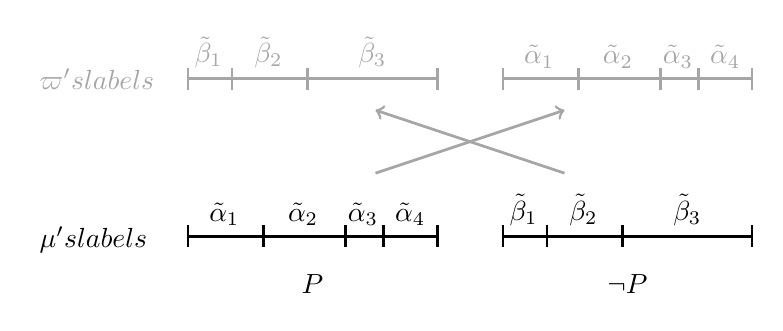
\begin{tikzpicture}[line width =1pt, scale=0.8]%[line cap=round,line join=round,>=triangle 45,x=1cm,y=1cm]
%\clip(-2.5,-2.15) rectangle (9.7,5.1);

\draw (-2.5,0.32) node[anchor=north west] {$\mu\text{'s labels}$};

\draw (0,0) -- (4,0) node[midway, below = 10pt]{$P$};
\draw [|-] (0,0) -- (1.2,0) node[midway, above]{$\small\tilde{\alpha}_1$};
\draw [|-] (1.2,0) -- (2.5,0) node[midway, above]{$\small\tilde{\alpha}_2$};
\draw [|-] (2.5,0) -- (3.1,0) node[midway, above]{$\small\tilde{\alpha}_3$};
\draw [|-|] (3.1,0) -- (4,0) node[midway, above]{$\small\tilde{\alpha}_4$};

\draw (5,0) -- (9,0) node[midway, below = 10pt]{$\lnot P$};
\draw [|-] (5,0) -- (5.7,0) node[midway, above]{$\small\tilde{\beta}_1$};
\draw [|-] (5.7,0) -- (6.9,0) node[midway, above]{$\small\tilde{\beta}_2$};
\draw [|-|] (6.9,0) -- (9,0) node[midway, above]{$\small\tilde{\beta}_3$};

\begin{scope}[color = aqaqaq]
\draw (-2.5,2.82) node[anchor=north west] {$\varpi\text{'s labels}$};

\draw [|-] (0,2.5) -- (0.7,2.5) node[midway, above]{$\small\tilde{\beta}_1$};
\draw [|-] (0.7,2.5) -- (1.9,2.5) node[midway, above]{$\small\tilde{\beta}_2$};
\draw [|-|] (1.9,2.5) -- (4,2.5) node[midway, above]{$\small\tilde{\beta}_3$};

\draw [|-] (5,2.5) -- (6.2,2.5) node[midway, above]{$\small\tilde{\alpha}_1$};
\draw [|-] (6.2,2.5) -- (7.5,2.5) node[midway, above]{$\small\tilde{\alpha}_2$};
\draw [|-] (7.5,2.5) -- (8.1,2.5) node[midway, above]{$\small\tilde{\alpha}_3$};
\draw [|-|] (8.1,2.5) -- (9,2.5) node[midway, above]{$\small\tilde{\alpha}_4$};

\draw [->] (6,1) -- (3,2);
\draw [->] (3,1) -- (6,2);
\end{scope}

\end{tikzpicture}
    \caption{Illustration of $\varpi$'s player countering $\mu$}
    \label{nonvf:fig:matchup}
\end{figure}

\subsection{Results}
\label{nonvf:sec:results}

\begin{definition}[Exploitation]
    An agent $\agent$ is said to \emph{exploit} a price-setter $\agent[p]$ if $\{\inventory(t,\top):t\in\Nats\}$ is bounded from below but not bounded from above.
    \label{nonvf:def:exploit}
\end{definition}

\begin{lemma}[Inexploitabity]
    There is no agent $\agent\in\agent[s]$ that exploits $\agent[pp]$.
    \label{nonvf:lem:inexploit}
\end{lemma}
\begin{proof}
    If any $\agent\in\agent[s]$ exploits $\agent[pp]$, then so does $\agent[m]$ (because the inventory allocated to $\agent$ will increase without bound, while all other agents' inventories are bounded below by 0 since they can only spend from their alloted inventory). However, by construction, $\agent[m]$ does not exploit $\agent[pp]$ (as it always holds an equal number of $P$ and $\lnot P$ stocks, and wins exactly as many games as it loses). Thus, no $\agent\in\agent[s]$ exploits $\agent[pp]$.
\end{proof}

\begin{theorem}[Convergence]
    $\lim_{t\to\infty}\price[pp](t,P)$ exists for all $P$; denote this as $\longrun(P)$.
    \label{nonvf:thm:convergence}
\end{theorem}
\begin{proof}
    Suppose it didn't; then there exists $x\in(0,1)$ and $\varepsilon>0$ such that $\price[pp](t,P)>x+\varepsilon$ infinitely often and $\price[pp](t,P)<x-\varepsilon$ infinitely often. Then consider an agent given by a trader that sells when $\price[pp](t,P)>x+\varepsilon$ and buys when $\price[pp](t,P)<x-\varepsilon$, and a trivial player (doesn't play at all; returns $\zero$ each time). This agent exploits the market.
\end{proof}

Ideally, we would like to say that our market learns to correctly price very FOL sentence: that $P$ is equivalent to $\longrun(t,P)=1$, and $\lnot P$ is equivalent to $\longrun(t,P)=0$: because if a true sentence did not approach \$1, an agent could buy arbitrarily large quantities of it and win the VF game on them. However, we know from Theorem~\ref{nonvf:thm:nogo} that this is impossible: indeed, the flaw in our intuition is that the mere existence of a winning strategy (i.e. the ``truth'' of $P$) does not imply it is actually computable. Instead, we adopt the following ``constructivist'' notion of truth, closely related to the notion of ``CGTS-truth'' (``Computational Game Theoretic Semantics Truth'') proposed in \cite{boyerProofTruth2012b}.

\begin{definition}[Constructive truth]
    Denote $\instaplayer[s]:=\Props\toc\finset\Nats$. For any $P\in\Props$ and $\instaplayer,\instaplayer[b]\in\instaplayer[s]$, observe that the sequence $\play{P}{\instaplayer,\instaplayer[b],\instaplayer,\instaplayer[b],\dots}$ eventually converges to a $\Delta_0$ sentence: denote this sentence by $\playfull(P,\instaplayer,\instaplayer[b])$. Then an FOL-sentence $P$ is said to be $\instaplayer[s]$-true if $\exists\instaplayer\in\instaplayer[s],\forall\instaplayer[b]\in\instaplayer[s],\playfull(P,\instaplayer,\instaplayer[b])$, and $\instaplayer[s]$-false if $\exists\instaplayer[b]\in\instaplayer[s],\forall\instaplayer[a]\in\instaplayer[s],\lnot\playfull(P,\instaplayer,\instaplayer[b])$.
    \label{nonvf:def:constructive}
\end{definition}

\begin{lemma}[Correspondence between $\instaplayers$ and $\players$]
    For any $\instaplayer:\Props\toc\finset\Nats$ there is a corresponding $\player:t\mapstopt\Props\too\strings\too\moves$ that executes it,, such that the following conditions are met: (1) $\forall s\ne t,\supp\instaplayer(t)\cap\supp\instaplayer(s)=\varnothing$ and (2) if $P\in\supp\instaplayer$ ($\instaplayer$ halts on input $P$) then $\exists t,\player(t,P,\foo)=\instaplayer(P)$ else $\forall t,\player(t,P,\foo)=\zero$.
    \label{nonvf:lem:correspondence}
\end{lemma}
\begin{proof}
    Fix an enumeration of $\Props$ i.e. a bijection $\zeta:\Nats\to\Props$, and fix a model of computation for $\instaplayer$, e.g. a Turing Machine. Then define $\player$ as follows:
    \begin{equation*}
        \player(t,P,l)=
        \begin{cases}
            \instaplayer(P) & \text{if } P\in\{\zeta(0),\dots,\zeta(t)\},\\&\ \ \ %
            \halts(\instaplayer,P,t),\\&\ \ \ \:%
            l=\foo \\
            \zero & \text{else}
        \end{cases}
    \end{equation*}
\end{proof}

\begin{theorem}[Learning constructive truth]
    If $P$ is an $\instaplayer[s]$-true sentence, then $\longrun(P)=1$.
    \label{nonvf:thm:main}
\end{theorem}
\begin{proof}
    Suppose it wasn't; then there is some $\varepsilon$ such that $\price[pp](t,P)$ is below $1-\varepsilon$ infinitely many times. Then consider the agent given by (1) the trader $\trader$ that buys whenever $\price[pp](t,P)<1-\varepsilon$ (2) the player $\player$ that is the Lemma~\ref{nonvf:lem:correspondence}-correspondent of the $\instaplayer$ affirmed in the hypothesis $\exists\instaplayer\in\instaplayer[s],\forall\instaplayer[b]\in\instaplayer[s],\playfull(P,\instaplayer,\instaplayer[b])$ (3) the labeler $\labeler$ that returns $\foo$ on all outputs. This agent exploits the market.
\end{proof}

\begin{corollary}[Learning constructive falsehood]
    If $P$ is an $\instaplayer[s]$-false sentence, then $\longrun(P)=0$.
    \label{nonvf:cor:main}
\end{corollary}
\begin{proof}
    Apply Thm~\ref{nonvf:thm:main} to $\lnot P$.
\end{proof}

% (L) closing remarks of the long version's Discussion that pertain
% specifically to the program-market results; the remainder of that
% paragraph (the alternate sigma-algebra proposal) is deduplicated
% into Section \ref{nonvf:sec:conclusion}.
We have presented a prediction market on sentences expressible in First-Order Logic and proven that our framework learns a notion of ``$\instaplayer[s]$-truth'' in the form presented in Def~\ref{nonvf:def:constructive}. However, our result (Thm~\ref{nonvf:thm:main}) is still somewhat weak, in that it says nothing about sentences that are neither $\instaplayer[s]$-true nor $\instaplayer[s]$-false -- from Thm~\ref{nonvf:thm:convergence}, we know that the market price of every sentence converges to \emph{something}, and it would be interesting to study the nature of this limiting distribution.

\section{Computational limitations}
\label{nonvf:sec:complexity}

There are two practical limitations of our work:
\begin{enumerate}
  \item Each player's move can be a finite set of arbitrary size, and the player is incentivized to play larger and larger finite sets. In particular, the final $\Delta_0$ sentence will be a disjunctive normal form over a very large number of $\Delta_0$ sentences, and getting the ground truth evaluations for all of them may take a long time (or cost a lot in computation).
  \item We have not considered computational costs of playing the VF game; the $\sup$ and $\inf$ in Theorem~\ref{nonvf:thm:supinf} are over all possible policies, even non-computable ones. In particular, the computational difficulty of playing for each side might be \emph{asymmetric}.
\end{enumerate}

For the first, we may charge a transaction cost proportional to the cardinality of the chosen move $S$ to incentivize agents to be selective in choosing the members of $S$ -- alternatively we may add a common discounting factor to the reward that would also disincentivize agents from choosing moves that would take a long time for their opponent to respond to. In the market mechanisms, we can also allow the agents to sell their place in the game to another agent at any point in time, so they do not need to wait for ground truth to be revealed to collect their reward.

The second is more serious: a classic example in game semantics \cite{solovievVerifierFalsifierGamesRestrictions2022} is the sentence $\exists x,\forall y,y\le\Ack(x)$ where $\Ack$ is the Ackermann function, and the class of policies is limited to primitive recursive functions (i.e. all other functions are infinitely expensive to play). Although this sentence is ``obviously'' false, $V$ can pick any $S$, and $F$ will be unable to win because the Ackermann function grows faster than all primitive recursive functions. In our case, it is apparent that if we took the $\sup_{\pi_V}$ and $\inf_{\pi_F}$ in Theorem~\ref{nonvf:thm:supinf} to be over primitive recursive functions only, the lower and upper bounds are both $1$, though $\Prob{P}$ should be 0 as $P$ is false.

One solution may come from the ``favourable'' games mentioned in Def~\ref{nonvf:def:vfgame}. In the example above, the falsifier has a winning strategy in the $F$-favourable game by indefinitely trying larger and larger integers as its move until it wins.

More generally, if we restrict the class of allowable policies to some $\Compcl\subset(\Props\to\finset\Nats)$, the $V$-favorable (respectively $F$-favourable) game still allows the $\sup$ (respectively $\inf$) to be taken over all of $\Props\to\finset\Nats$, as that player can simply enumerate each possible strategy. In general, we may play both the $F$-favorable and $V$-favorable games, and the range between the values of these games contains the range in Theorem~\ref{nonvf:thm:supinf}:

\begin{align}
&\sup_{\pi_V\in\Compcl}\inf_{\pi_F}\Prob{P[\pi_V,\pi_F]}\nonumber\\
&\le
\sup_{\pi_V}\inf_{\pi_F}\Prob{P[\pi_V,\pi_F]}\nonumber\\
&\le
\Prob{P}\label{nonvf:eq:bounds}\\
&\le
\inf_{\pi_F}\sup_{\pi_V}\Prob{P[\pi_V,\pi_F]}\nonumber\\
&\le
\inf_{\pi_F\in\Compcl}\sup_{\pi_V}\Prob{P[\pi_V,\pi_F]}\nonumber
\end{align}

Other approaches might be inspired by the Debate literature, for example \cite{brown-cohenScalableAISafety2023} introduces a version of the Debate protocol called ``Doubly-efficient debate'', where the honest strategy wins ``even when the debater is computationally unbounded''. Extending this to VF games should be a topic of future research.

% (L) the following paragraph is from the long version's Discussion
% (its practical-markets half; the applications sentence that opened
% it is placed in Section \ref{nonvf:sec:conclusion}).
With practical markets, however, special attention must be taken to take into account asymmetries in the computational costs of players for opposing sides: in our theoretical framework, every possible player was enumerated in the market, however practically some players may be ``more expensive'' than others, and this may influence how much traders are willing to pay for a side. For example, this may be addressed by ``separating out'' the market for players from the prediction market, so that traders are explicitly paying a price for purchasing players and this price can be added to the probability estimate for a sentence. In particular, this might also make it feasible to implement such systems with an automated market maker (e.g. logarithmic market scoring \cite{hansonLogarithmicMarketScoring2002, hansonCombinatorialInformationMarket2003}), as the obstacle to doing this immediately with our framework is that it's not obvious what player such a market-maker would use.

It remains unclear how much of a problem these computational limitations will be in practice.

\section{Discussion and future work}
\label{nonvf:sec:conclusion}

We have presented the ``ranged Verification-Falsification game'' and demonstrated that eliciting agents' values for playing this game provides useful bounds on the probability of an FOL sentence. Although usually applied to mathematical logic, FOL can also express sentences about some empirical universe, even if the process that generates empirical truth is probabilistic in nature. Our mechanism stands as an alternative framework to \cite{garrabrantLogicalInduction2020} for logical uncertainty, as well as the first mechanism to elicit probabilities on non-VF sentences from markets and AI models outside of a strict logical context. % (L) next sentence from the long version's Discussion:
Our work has a range of applications: the straightforward ones are to the study of logical uncertainty and relatedly bounded rationality, and to designing actual practical prediction markets for such sentences (e.g. prediction markets for various practically relevant statistical questions may be expressed in terms of limiting distributions of experimental results, thus as $\Pi_3$ sentences). There are three other potential implications of our work deserving of attention.

\textbf{Formal logic.} Our work may provide a new approach to measuring the strength of a mathematical theory: in the $V$-favourable VF game, a formal proof from a mathematical theory gives a computable winning strategy \cite{bonnayPreuvesJeuxSemantiques2004, boyerProofTruth2012}; we my then consider the maximum wealth that can be acquired by an agent that only trades and plays in accordance with a theory, and regard this as a measure of the strength of the theory.

\textbf{Eliciting latent knowledge.} Though we have used ``non-VF'' to refer specifically to FOL sentences, these are not the only sentences whose truth cannot be ascertained by ground truth. Take e.g. the sentence ``Bob did the crime''. This will not in itself be revealed by any future empirical observation, but may ``correlate'' with (provide information on) other, more directly valuable sentences like ``if Bob is jailed, fewer burglaries will happen'', ``evidence of Bob's wrongdoings will be found'' and ``if you hire Bob, you may find some office supplies missing''. One may say that these useful sentences are all correlated, and therefore ``Bob did the crime'' is a useful fiction constructed to capture the signal in the noisy data, a \emph{variable in the latent space}. The problem of eliciting information on such sentences has been discussed in e.g. \cite{tailcalledLatentVariablesPrediction2023, baillonBayesianMarketsElicit2017, baillonSimpleBetsElicit2021}, and directly addresses the problem of \emph{interpretability} in AI safety \cite{christianoElicitingLatentKnowledge2021}. We hope our work may serve as an entrypoint towards solving this much more ambitious goal. % (L) closing sentence from the long version's Discussion:
A comprehensive framework to address bets on such variables -- i.e. a market that decides what variables should exist in the latent space, then provides arbitration for betting on them -- would serve essentially the same function as an intelligent agent.

\textbf{Alternative formulations of probability theory.} It would be interesting to study what the elicited probabilities in these mechanisms actually approach in the limit, more precisely than the bounds in Equation~\ref{nonvf:eq:bounds}, e.g. when training AI forecasters (where $\Compcl$ would be the class of functions approximable by a neural network) or with a double auction containing every computable function in some class (e.g. those computable in polynomial-time) included as a trader by eventual enumeration. This would induce some ``distribution'' over the FOL algebra, which would \emph{not} be a probability distribution in the traditional sense (would not satisfy continuity of probability), as this would contradict Theorem~\ref{nonvf:thm:nogo}. Instead we might consider an alternate definition of a $\sigma$-algebra $\mathcal{F}$ which is required to be closed only under unions and intersections of \emph{computable sequences}, i.e. replacing the countable union axiom with ``$\psi:\Nats\to_{\Compcl}\mathcal{F}\implies\bigcup_i\psi(i)\in\mathcal{F}$'' (where $\Compcl$ is some class of computable functions) and adopting a suitable generalized notion of probability measure on this algebra. Possibly relevant work to this end includes: quantifier algebras \cite{cwooQuantifierAlgebra2013}, Shafer \& Vovk's game-theoretic formulation of probability theory \cite{shaferProbabilityFinanceIts2005, shaferGameTheoreticFoundationsProbability2019} and Japaridze's ``Computability Logic'' \cite{japaridzeBeginningWasGame2009, japaridzeSurveyComputabilityLogic2015}.

% ============================================================
% Subappendix: the long version's appendix on Garrabrant
% induction, using the fuller text of nonvf-paper-succint/
% stuff.tex (Section 1.1 there), which is a superset of the long
% version's appendix and also contains the long version's
% introduction's list of limitations of Garrabrant induction.
% ============================================================
\begin{subappendices}

\section{Garrabrant induction}
\label{nonvf:app:garrabrant}

A related problem is that of assigning probabilities to sentences of formal mathematics, i.e. \emph{logical uncertainty}. While this neither subsumes nor is subsumed by our problem (there are non-FOL mathematical theories, and conversely we may consider FOL sentences over e.g. empirical events rather than a formal language), there is substantial overlap, and it is worth considering if the methods in that area can be transferred to our problem. The crown jewel of the logical uncertainty literature, \emph{Garrabrant induction} \cite{garrabrantLogicalInduction2016}, in fact implements a prediction market for all logical sentences which pays off whenever a sentence is proven by some formal theorem prover (which exists for any ``computably enumerable theoory'', including first-order arithmetic etc.). However, this would simply be a prediction market for the \emph{provability} of a sentence (in some particular formal theory); the actual Garrabrant induction framework instead adopts a notion of ``propositionally consistent worlds'' that allows even unprovable (and provably unprovable) sentences to have non-zero probabilities and such that basic probabilistic laws like $\Prob{P}+\Prob{\lnot P}=1$ are followed.

The idea is as follows: if $P\lor Q$ is proven, then an agent that holds a stock each in sentences $P$ and $Q$ must necessarily be regarded as having \emph{at least} \$1 between these assets. Similarly if $\lnot P\lor\lnot Q$ is proven, then that agent has \emph{at most} \$1 between these assets. We call these different logical possibilities ``worlds'' or rather ``worlds that are propositionally consistent with the output of the theorem prover so far'' (PC worlds for short). In particular when evaluating whether a trade is within budget (to be accepted by the market-maker), we demand that it is within budget in all PC worlds. More precisely:

\begin{definition}[Worlds and valuations]
    Let $\inventory:\Props\too\Rats$ be a finite-supported map, and let $\world:\Props\to\Bools$ be a \emph{world}, i.e. a truth-assignment, so the dot product $\world\cdot\inventory$ represents the valuation of $\inventory$ according to $\world$.
\end{definition}

\begin{definition}[PC worlds]
     A world is said to be propositionally consistent (PC) if for all $P\in\Props$, $\world(P)$ is determined by Boolean algebra from the prime sentences in $\Props$, i.e. $\world(P\land Q)=\world(P)\land \world(Q)$, $\world(P\lor Q)=\world(P)\lor \world(Q)$, etc. Furthermore, let $\thms_t$ be the subset of $\Props$ proven by time $t$: then a world is said to be PC with $\thms_t$ if (1) it is PC and (2) $\world(P)=1$ for all $P\in\thms_t$. We denote the set of worlds PC with $\thms_t$ as $\PC(\thms_t)$; in particular $\PC:=\PC(\{\})$. For any $\inventory$, denote its set of plausible valuations as $\PC(\thms_t,\inventory):=\{\world\cdot\inventory\mid \world\in\PC(\thms_t)\}$.
\end{definition}

Note that $\PC(\thms_t,\inventory)$ is computable, since you only have to check propositional consistency for the sentences actually supported by $\inventory$.

Another quirk of Garrabrant induction is that agents have type $\agent:\Nats\to(\Props\to\probs)\to(\Props\to\Rats)$ i.e. they output ``joint'' demand schedules allowing for cross-elasticity of demand rather than leaving this to be figured out by the market dynamics. Naturally, calculating equilibrium between such demand schedules is non-trivial and requires Brouwer's fixed point theorem, as well as constraints on $\agent$ (specifically that $\agent(t)$ is continuous in price and comprised only of some particularly simple expressions depending only on some external information like price history). The framework actually implements a rational approximation of the equilibrium computed via a brute-force Farey enumeration of all rational numbers.

\begin{definition}[Garrabrant induction]
    Fix a language $\Props$, a theorem enumerator $\thms:\Nats\to\finset\Props$ (obeying in particular $s\le t\implies\thms_s\subseteq\thms_t$) and enumerator of agents $\father:\Nats\to\agent[s]\times\Rats$ such that $\father_1$ is bijective and $\sum_t\father_2(t)<\infty$ (where $\father=(\father_1,\father_2)$ and $\agent[s]$ is the type specified earlier $\Nats\to(\Props\to\probs)\to(\Props\to\Rats)$). Then the Garrabrant induction algorithm is given by the following mutual recursion:
    \begin{itemize}
        \item an ``aggregate trader'' $$\agent[m](t,\pricee):=\sum_{\agent\in\{\father(1)\dots\father(t)\}}\indicate{\min\PC(\thms_t,\inventory(t,\pricee) + \agent(t,\pricee))\ge 0}\agent(t,\pricee)$$ where $\indicate{}$ denotes an indicator function
        \item an ``equilibrium price'' $\pricee(t)$, which approximates a zero of $\agent[m](t)$ i.e. so that $\agent[m](t,\pricee(t))\approx 0$ (in particular the error should be $\le 1/2^t$)
        \item an inventory account $\inventory(t,P)$, as computed by the following algorithm:
    \end{itemize}

    \begin{algorithm}
    \begin{algorithmic}
    \Function{$\inventory$}{$\tau$}
        \For{$t\le\tau$}
            \State $\inventory[\father_1(t)](\top)\gets\father(t)_2$
            \For{$X\in\supp{\inventory}$} \Comment{resolve proven sentences}
                \If{$X\in\thms_t$}
                    \State $\inventory(\top) \gets \inventory(\top)+\inventory(X)$
                    \State $\inventory(X)\gets 0$
                \EndIf
            \EndFor
            \For{$X\in\supp\agent$}
                \If{$\min\PC(\thms_t,\inventory(t,\pricee) + \agent(t,\pricee))\ge 0$}
                    \State $\inventory\gets\inventory+\agent(t)$ \Comment{add trade to inventory}
                \EndIf
            \EndFor
        \EndFor
        \State \Return $\inventory$
    \EndFunction
    \end{algorithmic}
    \end{algorithm}
    \label{nonvf:def:garrabrant}
\end{definition}

[A slight difference in the formulation we have presented is that we put the onus on the individual agents to calculate and include the cash payment within their orders, and the aggregate agent just zeroes their trade if they submit an invalid trade; this makes no difference to the whole algorithm.]

\begin{theorem}[Inexploitability]
    With definitions as in Def~\ref{nonvf:def:garrabrant}, \emph{no trader $\agent\in\agent[s]$ can exploit the price sequence $\pricee$}, i.e. $\PC(\thms_t,\inventory(t))$ remains bounded from above.
    \label{nonvf:thm:garrabrant}
\end{theorem}

\begin{hproof}
    If any trader could exploit the price sequence, so could the aggregate trader $\agent[m]$ (as whichever trader exploits the market would also grow its proportion of $\agent[m]$'s trades to $+\infty$, and no trader can run $\agent[m]$'s finances to $-\infty$ since it would just go bankrupt). However, $\agent[m]$ cannot exploit $\pricee$ as it is set to be (arbitrary close to) an equilibrium for $\agent[m]$.
\end{hproof}

Indeed, Garrabrant induction may be applied to some FOL theory and be seen as a competing framework to ours -- however, it has crucial limitations:
\begin{itemize}
    \item It does not exploit the \emph{FOL structure} of the language, so it doesn't tell us anything about the relationship between the sentences $P(x)$ and $\exists x, P(x)$ as e.g. probability theory would.
    \item It is fundamentally ``theory-dependent'', which leaves some foundational questions unanswered from a philosophical perspective: it doesn't address the question of \emph{why} we give credence to particular formal theories for forming our beliefs (ideally, our answer to this should look like ``because formal theories make a lot of money on the market''). Although this may seem like a rather detached philosophical problem, it is likely relevant should we seek to design intelligent agents that form beliefs about mathematical truths (for general examples of market-based designs of decision-making agents see \cite{oesterheldTheoryBoundedInductive2023, changDecentralizedReinforcementLearning2020, kweeMarketBasedReinforcementLearning2001, baumModelIntelligenceEconomy1999, balduzziCorticalPredictionMarkets2014}), as we would like the agent to be able to reflect beyond the computational limitations of a particular theory.
    \item It cannot be readily extended beyond the realm of formal logic: while \cite{garrabrantLogicalInduction2016} does make note that the framework performs something akin to empirical induction for sentences independent of a theory, this notion of empirical induction once again does not exploit the FOL structure of the language.
\end{itemize}

\end{subappendices}
